\chapter{The Conformal Frame and the Self-Dual Connection}\markboth{\MakeUppercase{Chapter 21.\ Conformal frame, self-dual connection}}{}
\label{ch:conformal}

\begin{usesbox}
\textbf{This chapter uses:} the hemisphere model and the Gudermannian (\cref{thm:hemibij,thm:gudermann}); the spin-connection condition $w=r'$ (\cref{thm:spinwitten}); the Misner--Sharp mass (\cref{prop:massprime}); the Tolman universe and the throat (\cref{thm:tolman,thm:br}); the global coordinates of $\mathrm{AdS}_2$ (\cref{prop:clocks}).\\
\textbf{It provides:} the Gauss map of a time-symmetric slice embedded in $\mathbb R^4$, whose polar height is $w=r'$ and whose angle measures the compactness, $\sin^2\chi=2Gm/r$; the conformal frame in which both the Tolman universe and the throat are conformal to the Einstein static universe $\mathbb R\times S^3$, with conformal factors $\ell\cos\eta$ and $\ell/\sin u$ solving one linear equation; the minisuperspace energy balance; and the self-dual (Ashtekar) connection of the Tolman universe, whose phase runs along the hemisphere of \cref{ch:hemisphere} from the pole to the equator.
\end{usesbox}

In \cref{ch:hemisphere} the states of a massive particle were points of a hemisphere, with height $m/E$. This chapter shows that the same hemisphere describes the glued spacetime in two further ways. On the initial slice it is the image of the Gauss map. During the evolution it is traced by the phase of the self-dual connection. In between, a conformal rescaling puts the Tolman universe and the throat on the same Einstein static universe, where they appear as a time-dependent and a space-dependent solution of one linear equation.

\section{The Gauss map of a spherical slice}

A time-symmetric slice $\dd s^2+r(s)^2\dd\Omega^2$ with $|r'|\le1$ can be realised as a hypersurface of revolution in Euclidean $\mathbb R^4$: put $X(s,\mathbf n)=(r(s)\mathbf n,z(s))$ with $\mathbf n\in S^2$ and $z(s)=\int_0^s\sqrt{1-r'(x)^2}\,\dd x$.

\begin{theorem}[Embedding and Gauss map]\label{thm:gaussmap}\ver\
\begin{enumerate}[label=(\roman*)]
\item $z$ is differentiable with $z'=\sqrt{1-r'^2}$, so $r'^2+z'^2=1$; $X$ is differentiable in $s$ and its derivatives are the expected tangent vectors. The induced metric is $\dd s^2+r^2\dd\Omega^2$. If $z$ is strictly increasing and $r\ne0$, the profile map is injective.
\item The vector $N=(-z'\mathbf n,r')$ is a unit vector orthogonal to all tangent vectors, and every unit vector with this property is $\pm N$ (for $r\ne0$).
\item Let $\chi$ be the angle between $N$ and the axis $e_4$. Then
\[
\cos\chi=r'=w,\qquad \sin^2\chi=1-r'^2=\frac{2Gm}r,
\]
where $m$ is the Misner--Sharp mass of the time-symmetric slice. In particular $\chi=\pi/2$ $\Leftrightarrow$ $r'=0$ $\Leftrightarrow$ $2Gm=r$, a marginally trapped sphere. For Schwarzschild, $1-(\sqrt{1-2m/r})^2=2m/r$.
\item On the Tolman side $\cos\chi=\cos(s/\ell)$, so $\chi=s/\ell$ for $0\le s\le\pi\ell/2$: the Gauss map is the identity of the hemisphere. On the throat $\chi=\pi/2$ throughout: the throat maps to the equator. The junction $s=\pi\ell/2$ is on the equator from both sides.
\end{enumerate}
\end{theorem}

\begin{proposition}[Principal curvatures]\label{prop:principal}\ver\
Let $k_r$ and $k_\perp$ be the principal curvatures of the embedded slice in the radial and angular directions. The time-symmetric Hamiltonian constraint ${}^{(3)}R=16\pi G\rho$ reads $2\sigma_2=16\pi G\rho$ with $\sigma_2=2k_rk_\perp+k_\perp^2$.
\begin{enumerate}[label=(\roman*)]
\item In vacuum ($\sigma_2=0$, $k_\perp\ne0$), $k_r/k_\perp=-\frac12$: the Flamm paraboloid.
\item For a star of uniform density, $k_r=k_\perp=c$ with $c^2=2M/R^3$ gives $\rho=3M/(4\pi R^3)$ (in units $G=1$): the interior is a piece of a round $S^3$.
\end{enumerate}
\end{proposition}

\begin{figure}[t]
\centering
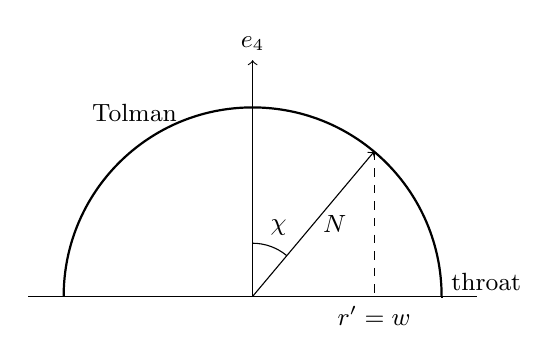
\begin{tikzpicture}[scale=1.5]
\draw[thick] (-1.6,0) arc (180:90:1.6) ;
\draw[thick] (0,1.6) arc (90:0:1.6);
\draw[thick] (1.6,0) -- (1.6,-0.01);
\draw (-1.9,0) -- (1.9,0);
\draw[->] (0,0) -- (0,2.0) node[above] {\small $e_4$};
\draw[->] (0,0) -- ({1.6*cos(50)},{1.6*sin(50)}) node[midway,right] {\small $N$};
\draw (0,0.45) arc (90:50:0.45);
\node at (0.22,0.58) {\small $\chi$};
\draw[dashed] ({1.6*cos(50)},{1.6*sin(50)}) -- ({1.6*cos(50)},0) node[below] {\small $r'=w$};
\node[right] at (1.6,0.12) {\small throat};
\node at (-1.0,1.55) {\small Tolman};
\end{tikzpicture}
\caption{The Gauss map of the glued slice. The unit normal $N$ makes the angle $\chi$ with the axis; its height is $\cos\chi=r'=w$ and $\sin^2\chi=2Gm/r$. The Tolman side covers the hemisphere once; the throat sits on the equator.}
\label{fig:gauss}
\end{figure}

\Cref{thm:gaussmap} gives the spin-connection condition $w=r'$ a geometric meaning: the Yang--Mills potential is the height of the unit normal. The compactness $2Gm/r$ is the square of the horizontal component. The pole is flat space, the equator is a horizon, and the glued slice runs from the pole to the equator and then stays there. This is the hemisphere of \cref{ch:hemisphere} once more, now with $2Gm/r$ in place of $|\mathbf p|^2/E^2$.

\section{Both pieces on the Einstein static universe}

Write the Tolman metric as $\Omega^2\hat g$ with $\Omega=\ell\cos\eta$ and $\hat g=-\dd\eta^2+\dd u^2+\sin^2u\,\dd\Omega^2$, the Einstein static universe of unit radius. The throat can be written in the same way: with $x=\ell\log\tan(u/2)$ one has $\dd x/\dd u=\ell/\sin u$, so
\[
-\dd t^2+\dd x^2+\ell^2\dd\Omega^2\ \to\ \frac{\ell^2}{\sin^2u}\bigl(-\dd\eta^2+\dd u^2+\sin^2u\,\dd\Omega^2\bigr),
\]
which is the global form of $\mathrm{AdS}_2\times S^2$ (\cref{prop:clocks}(iii)) and shows that the throat is conformal to $\hat g$ with $\Omega=\ell/\sin u$. As $x\to\pm\infty$ one approaches the poles $u=0,\pi$ of $S^3$.

Since Yang--Mills theory is conformally invariant, its stress tensor is traceless and every EYM solution has $R=0$. For $g=\Omega^2\hat g$ this is the conformally coupled wave equation $(\hat\Box-\hat R/6)\Omega=0$, which on the unit Einstein static universe ($\hat R=6$) reads
\begin{equation}\label{eq:confwave}
\hat\Box\,\Omega=\Omega,\qquad \hat\Box=-\partial_\eta^2+\Delta_{S^3}.
\end{equation}
This general fact is standard \ext; we verify it directly for the solutions at hand.

\begin{theorem}[One linear equation]\label{thm:confwave}\ver\
\begin{enumerate}[label=(\roman*)]
\item The Tolman factor $\Omega=\ell\cos\eta$ satisfies $-\ddot\Omega=\Omega$; every solution $A\cos\eta+B\sin\eta$ is $2\pi$-periodic.
\item The throat factor $\Omega=\ell/\sin u$ satisfies $\Omega''+2\cot u\,\Omega'=\Omega$, the radial part of $\Delta_{S^3}\Omega=\Omega$. More generally every static solution of the form $\Omega=(A+Bu)/\sin u$ satisfies it.
\item The $\eta\eta$ Einstein equation holds for the throat, $\Omega^2+\Omega'^2=\ell^2/\sin^4u=8\pi G/(2g^2\sin^4u)$, and for the Tolman universe, $3(\Omega^2+\dot\Omega^2)=3\ell^2=8\pi G\cdot3/(2g^2)$, in both cases exactly when $\ell^2=4\pi G/g^2$.
\item At the junction $u=\pi/2$, the throat has $\Omega=\ell$, $\Omega'=0$, $\Omega''=\ell$, while the time-symmetric Tolman slice has $\Omega=\ell$ and vanishing spatial derivatives: the join is a seam in the second derivative of the conformal factor.
\item The Yang--Mills potential is $w=r'=(\Omega'\sin u+\Omega\cos u)/\Omega$ (with $r=\Omega\sin u$, $\dd s=\Omega\,\dd u$), which is $0$ on the throat and $\cos u$ on the Tolman side.
\item The sum $\Omega=A\cos\eta+B/\sin u$ solves \eqref{eq:confwave}, but its null--null Einstein components acquire cross terms: they equal $4A^2+ABc(8-4w^2)w\pm8ABswt$ with $c=\cos\eta$, $s=\sin\eta$, $w=1/\sin u$, $t=\cot u$. The linear superposition is therefore not a solution unless $AB=0$.
\end{enumerate}
\end{theorem}

In the conformal frame the two pieces are the simplest possible solutions of \eqref{eq:confwave}: a homogeneous oscillation in time, and a static mode concentrated around the equator of $S^3$. The polar angle $u$ on $S^3$ plays the same role on both sides, and the junction is at $u=\pi/2$. The coordinate $x=\ell\log\tan(u/2)$ is again a Mercator coordinate: $\log\tan(u/2)$ is the inverse Gudermannian of $u-\pi/2$.

\begin{proposition}[Minisuperspace energy balance]\label{prop:minisuper}\ver\
For a homogeneous $\Omega(\eta)$ on $S^3$, the gravitational energy is $H_\Omega=-\frac{3\pi}{4G}(\dot\Omega^2+\Omega^2)$, which equals $-\frac{3\pi}{4G}\ell^2$ along the Tolman solution. The Yang--Mills energy on the unit $S^3$ is $E_{\rm YM}=3\pi^2/g^2$, and the Hamiltonian constraint $H_\Omega+E_{\rm YM}=0$ holds if and only if $\ell^2=4\pi G/g^2$.
\end{proposition}

The gravitational part is an oscillator with negative energy, the matter part a positive constant. This is the starting point for the canonical quantisation of Chapter~26.

\begin{proposition}[Where smooth static solutions go]\label{prop:extremallimit}\ver\
For $w=0$ and unit magnetic charge, $m(r)=1-1/(2r)$ satisfies $m'=(1-w^2)^2/(2r^2)$, and $N=1-2m/r=(1-1/r)^2$: the extremal Reissner--Nordstr\"om solution, with a degenerate horizon at $r=1=\ell$ whose near-horizon geometry is the throat.
\end{proposition}

The Bartnik--McKinnon solutions with $n$ nodes approach this extremal solution as $n\to\infty$ \cite{BFM1994} \ext. So the throat is also the limit of the smooth static family; we met the rate $e^{-\pi/\sqrt3}$ in \cref{thm:throatmode}.

\section{The self-dual connection of the Tolman universe}

For a closed FRW universe with scale factor $a$ and cosmic-time derivative $\dot a$, the self-dual Ashtekar connection is homogeneous and given by a single complex number $c=\Gamma+iK$, with spin-connection part $\Gamma=1$ and extrinsic-curvature part $K=\dot a$ \cite{Ashtekar1986,AshtekarPawlowskiSingh2006}. Its curvature is proportional to $c^2-2c$.

\begin{theorem}[Self-dual connection and the hemisphere]\label{thm:selfdual}\ver\
\begin{enumerate}[label=(\roman*)]
\item For $c=1+i\dot a$: $c^2-2c=-(1+\dot a^2)$ is real and $|c|^2=1+\dot a^2$. The Friedmann equation $\dot a^2+1=\frac{8\pi G}3\rho a^2$ is equivalent to $-(c^2-2c)=|c|^2=\frac{8\pi G}3\rho a^2$.
\item For the Tolman universe $a=\ell\cos\eta$: $\dot a=-\tan\eta$, $|c|^2=1/\cos^2\eta=\ell^2/a^2$, and with $\rho=3/(2g^2a^4)$ the right-hand side is $\ell^2/a^2$ exactly when $\ell^2=4\pi G/g^2$.
\item (Phase) $c\cos\eta=(1-i\tan\eta)\cos\eta=e^{-i\eta}$. At $\eta=0$, $c=1$ (pure rotation); as $\eta\to\pi/2$ the phase tends to $e^{-i\pi/2}=-i$ (pure boost).
\item (Mass shell) Write $\dot a=-\sinh\zeta$. Then $|c|^2=\cosh^2\zeta$; the normalised connection $c/|c|=(\operatorname{sech}\zeta,-\tanh\zeta)$ lies on the unit circle; and $(|c|,\operatorname{Im}c)=(\cosh\zeta,-\sinh\zeta)$ lies on the unit hyperbola. If $\tan\theta=\sinh\zeta$ with $\cos\theta>0$, then $\cos\theta=\operatorname{sech}\zeta$: $\theta=\gd\zeta$.
\item (Real part) The real part of $\Gamma+iK$ is the spin connection $\Gamma$. On the Tolman side the spin-connection potential of $r=a\sin\chi$, $\dd s=a\,\dd\chi$, is $w=r'=\cos\chi$, independent of $a$: it agrees with the Yang--Mills solution at every moment.
\item For the throat in synchronous coordinates, $K^z{}_z=-\tan(t/\ell)/\ell$; since only one component of $K$ is non-zero, $K^2-K_{ab}K^{ab}=0$ and the Hamiltonian constraint reduces to ${}^{(3)}R=16\pi G\rho$.
\end{enumerate}
\end{theorem}

Part (iv) is the dictionary of \cref{ch:hemisphere} read in cosmology. The real part of the connection, $\Gamma=1$, plays the role of the mass; the imaginary part, $\dot a$, plays the role of the momentum; $|c|$ is the energy. The hemisphere point $(m/E,p/E)$ becomes $(\cos\eta,-\sin\eta)$ and the Gudermannian relates the conformal time $\eta$ to the ``rapidity'' $\zeta$ of the expansion. The life of the Tolman universe, from maximal expansion to the crunch, is the passage along a meridian of the hemisphere from the pole, where the particle is at rest, to the equator, where it moves at the speed of light. The Yang--Mills field is the real part of the self-dual connection and stays fixed, $w=\cos\chi$, during the whole passage.

\begin{litbox}
Embeddings of spherically symmetric slices, the Flamm paraboloid and the relation $\sin^2\chi=2Gm/r$ for the Schwarzschild slice are classical \cite{MTW}; the conformal wave equation and the Einstein static universe as conformal compactification are standard \cite{HawkingEllis,PenroseRindler1}; the self-dual connection is Ashtekar's \cite{Ashtekar1986}, and its use in homogeneous cosmology is the basis of loop quantum cosmology \cite{AshtekarPawlowskiSingh2006}. What is new here is the following: the Gauss map of the glued slice, with $w=r'$ as the height of the normal, the Tolman side covering a hemisphere and the throat on the equator (\cref{thm:gaussmap}); the presentation of the Tolman universe and the Bertotti--Robinson throat as a time-dependent and a space-dependent solution of the same conformal wave equation on $\mathbb R\times S^3$, joined at the equator $u=\pi/2$ (\cref{thm:confwave}); and the identification of the phase of the Tolman self-dual connection with the hemisphere point of a massive particle via the Gudermannian (\cref{thm:selfdual}).
\end{litbox}

\section*{What this chapter passes on}
\begin{itemize}[nosep]
\item Gauss map: $\cos\chi=w=r'$, $\sin^2\chi=2Gm/r$ (\cref{thm:gaussmap}).
\item Both pieces on $\mathbb R\times S^3$: $\ell\cos\eta$ and $\ell/\sin u$ solve $\hat\Box\Omega=\Omega$ (\cref{thm:confwave}).
\item Energy balance $-\frac{3\pi}{4G}\ell^2+\frac{3\pi^2}{g^2}=0$ (\cref{prop:minisuper}).
\item Self-dual connection $c=1+i\dot a$ with $c\cos\eta=e^{-i\eta}$, tracing the hemisphere (\cref{thm:selfdual}).
\end{itemize}

\section*{Exercises}
\begin{exercise}
Show that $x=\ell\log\tan(u/2)$ satisfies $\dd x/\dd u=\ell/\sin u$ for $0<u<\pi$.
\end{exercise}
\begin{exercise}
Verify that $\Omega=\ell/\sin u$ satisfies $\Omega''+2\cot u\,\Omega'=\Omega$.
\end{exercise}
\begin{exercise}
Show $(1-i\tan\eta)\cos\eta=e^{-i\eta}$ and $|1+i\dot a|^2=1+\dot a^2$.
\end{exercise}
\begin{exercise}
For vacuum, show that $2k_rk_\perp+k_\perp^2=0$ with $k_\perp\ne0$ forces $k_r/k_\perp=-\frac12$.
\end{exercise}

\begin{checklist}
\chk{AlphaV_GaussMap:ip_smul_left,AlphaV_GaussMap:ip_smul_right,AlphaV_GaussMap:ip_comm}{Elementary properties of the inner product (three lemmas).}
\chk{AlphaV_GaussMap:X_deriv}{Derivative of the embedding.}
\chk{AlphaV_GaussMap:embed_exists}{The height function and $r'^2+z'^2=1$.$^*$}
\chk{AlphaV_GaussMap:profileMap_injective}{Injectivity of the profile map.$^*$}
\chk{AlphaV_GaussMap:embed_metric}{Induced metric $\dd s^2+r^2\dd\Omega^2$.$^*$}
\chk{AlphaV_GaussMap:profile_immersion_data}{Combined immersion statement.$^*$}
\chk{AlphaV_GaussMap:normal_unit,AlphaV_GaussMap:normal_orth,AlphaV_GaussMap:normal_unique}{The unit normal and its uniqueness up to sign (three statements).$^*$}
\chk{AlphaV_GaussMap:gauss_cos}{$\cos\chi=r'$.$^*$}
\chk{AlphaV_GaussMap:gauss_sin_mass}{$\sin^2\chi=2Gm/r$.$^*$}
\chk{AlphaV_GaussMap:gauss_equator}{Equator $\Leftrightarrow$ $2Gm=r$.$^*$}
\chk{AlphaV_Gauss:gauss_normal,AlphaV_Gauss:gauss_angle,AlphaV_Gauss:gauss_mass}{Pointwise normal, angle and mass relations (three statements).}
\chk{AlphaV_Gauss:gauss_schwarzschild,AlphaV:gauss_compactness}{Schwarzschild: $1-(\sqrt{1-2m/r})^2=2m/r$ (two statements).}
\chk{AlphaV_Gauss:gauss_marginal}{Equator $\Leftrightarrow$ $r'=0$ $\Leftrightarrow$ $2Gm=r$.}
\chk{AlphaV_Gauss:gauss_cap,AlphaV_Gauss:gauss_neck}{Gauss angle $\chi=s/\ell$ on the Tolman side and $\pi/2$ on the throat (two statements).$^*$}
\chk{AlphaV:gauss_vacuum}{Vacuum: $k_r/k_\perp=-\frac12$.$^*$}
\chk{AlphaV:gauss_interior}{Uniform-density interior.$^*$}
\chk{AlphaPillar_Conformal:neck_coordinate}{$x=\ell\log\tan(u/2)$ and the conformal form of the throat.$^*$}
\chk{AlphaPillar_Conformal:cap_box,AlphaPillar_Conformal:periodic}{$-\ddot\Omega=\Omega$ for the Tolman factor; periodicity (two statements).$^*$}
\chk{AlphaPillar_Conformal:neck_derivs,AlphaPillar_Conformal:neck_box}{$\Omega''+2\cot u\,\Omega'=\Omega$ for $\ell/\sin u$ (two statements).$^*$}
\chk{AlphaPillar_Conformal:static_general,AlphaPillar_Conformal:static_general_deriv}{Static solutions $(A+Bu)/\sin u$ (two statements).$^*$}
\chk{AlphaPillar_Conformal:eta_neck,AlphaPillar_Conformal:eta_cap}{The $\eta\eta$ Einstein equation on both sides (two statements).$^*$}
\chk{AlphaPillar_Conformal:junction_seam}{The seam at $u=\pi/2$.$^*$}
\chk{AlphaPillar_Conformal:r_prime_conformal}{$w=r'$ in the conformal frame.$^*$}
\chk{AlphaPillar_Smooth:superpos_null}{Null components of the superposition.$^*$}
\chk{AlphaPillar_Conformal:cap_energy,AlphaPillar_Conformal:energy_balance}{Minisuperspace energy and the Hamiltonian constraint (two statements).$^*$}
\chk{AlphaPillar_Conformal:extremal_limit}{Extremal RN with $m'=(1-w^2)^2/(2r^2)$.$^*$}
\chk{AlphaPillar_SelfDual:curvature_real,AlphaPillar_SelfDual:norm_c}{$c^2-2c=-(1+\dot a^2)$ and $|c|^2=1+\dot a^2$ (two statements).}
\chk{AlphaPillar_SelfDual:friedmann_selfdual}{Friedmann in self-dual form.$^*$}
\chk{AlphaPillar_SelfDual:cap_hubble,AlphaPillar_SelfDual:cap_modulus,AlphaPillar_SelfDual:cap_rhs}{Tolman: $\dot a=-\tan\eta$, $|c|^2=\ell^2/a^2$, and the right-hand side (three statements).$^*$}
\chk{AlphaPillar_SelfDual:phase_lemma,AlphaPillar_SelfDual:end_phase}{Phase $e^{-i\eta}$ and its end values (two statements).$^*$}
\chk{AlphaPillar_SelfDual:mass_shell}{Circle and hyperbola: the hemisphere and the mass shell.$^*$}
\chk{AlphaPillar_SelfDual:gudermann_phase}{$\theta=\gd\zeta$.$^*$}
\chk{AlphaPillar_SelfDual:real_part,AlphaPillar_SelfDual:cap_real_part}{Real part is the spin connection; $w=\cos\chi$ independent of $a$ (two statements).$^*$}
\chk{AlphaPillar_SelfDual:neck_extrinsic,AlphaPillar_SelfDual:neck_constraint}{Throat extrinsic curvature and constraint (two statements).}
\end{checklist}
